\section{安装Spark}
\subsection{简介}
Spark是一个内存计算框架,其速度能够在很大程度上
超过Hadoop的Mapreduce,并逐渐取代其,在大数据分析和处理上占据了重要的地位。
Spark的安装有本地模式安装、Standalone模式安装和集群模式安装。集群模式需要
借助YARN或Meso,而且与Stadalone模式配置类似。这里采用Spark on YARN实现集群。

\subsection{通过SDKMAN安装Scala}
运行Spark或者Spark开发需要Scala运行环境,这里采用了官网推荐的通过SDKMAN方法安装。
当然也可以采用下载二进制包然后配置环境变量的方式,不过多描述。

\begin{lstlisting}[style=mysh,title=安装Scala]
$ sudo apt install curl
$ curl -s "https://get.sdkman.io" | bash
# this take a while
$ source ~/.bashrc
$ sdk install scala
# 查看scala所在的目录
$ whereis scala
# 将其配置到.bashrc环境变量中
# 输入scala进行测试
$ scala
scala> 
\end{lstlisting}
\subsection{配置文件}
在安装好Scala和具备Hadoop环境后,即可进行Spark的安装和部署。
\lstinputlisting[style=mysh,title=spark-env.sh]{docs/spark/conf/spark-env.sh}
\lstinputlisting[style=mysh, title=slaves]{docs/spark/conf/slaves}
而且可以设置\lstinline{log4j.properties.template}文件设置输出日志级别,
避免打印过多的INFO级别的日志信息。
\subsection{测试Spark Shell}
Spark shell是一个特别适合快速开发Spark程序的工具。即使你对Scala不熟悉,仍然可以使用这个工具快速应用Scala操作Spark。
Spark shell使得用户可以和Spark集群交互,提交查询,这便于调试,也便于初学者使用Spark。
Spark shell是非常方便的,因为它很大程度上基于Scala REPL(Scala交互式shell,即Scala解释器),并继承了Scala REPL(读取-求值-打印-循环)(Read-Evaluate-Print-Loop)的所有功能。运行spark-shell,则会运行spark-submit,spark-shell其实是对spark-submit的一层封装。

下面是Spark shell的运行原理图

\begin{figure}[htbp]
    \centering
    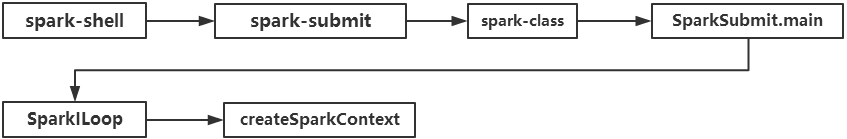
\includegraphics[width=\linewidth]{spark/spark-shell.png}    
    \caption{Spark shell的运行原理图}
    \label{fig:spark_shell}
\end{figure}
RDD有两种类型的操作 ,分别是Transformation(返回一个新的RDD)和Action(返回values)。
\begin{itemize}
    \item Transformation:根据已有RDD创建新的RDD数据集build

\begin{enumerate}[1)]
\item map(func):对调用map的RDD数据集中的每个element都使用func,然后返回一个新的RDD,这个返回的数据集是分布式的数据集。
\item filter(func) :对调用filter的RDD数据集中的每个元素都使用func,然后返回一个包含使func为true的元素构成的RDD。
\item flatMap(func):和map很像,但是flatMap生成的是多个结果。
\item mapPartitions(func):和map很像,但是map是每个element,而mapPartitions是每个partition。
\item mapPartitionsWithSplit(func):和mapPartitions很像,但是func作用的是其中一个split上,所以func中应该有index。
\item sample(withReplacement,faction,seed):抽样。
\item union(otherDataset):返回一个新的dataset,包含源dataset和给定dataset的元素的集合。
\item distinct([numTasks]):返回一个新的dataset,这个dataset含有的是源dataset中的distinct的element。
\item groupByKey(numTasks):返回(K,Seq[V]),也就是Hadoop中reduce函数接受的key-valuelist。
\item reduceByKey(func,[numTasks]):就是用一个给定的reduce func再作用在groupByKey产生的(K,Seq[V]),比如求和,求平均数。
\item sortByKey([ascending],[numTasks]):按照key来进行排序,是升序还是降序,ascending是boolean类型。
\end{enumerate}
\item  Action:在RDD数据集运行计算后,返回一个值或者将结果写入外部存储
\begin{enumerate}[1)]
\item reduce(func):就是聚集,但是传入的函数是两个参数输入返回一个值,这个函数必须是满足交换律和结合律的。
\item collect():一般在filter或者足够小的结果的时候,再用collect封装返回一个数组。
\item count():返回的是dataset中的element的个数。
\item first():返回的是dataset中的第一个元素。
\item take(n):返回前n个elements。
\item takeSample(withReplacement,num,seed):抽样返回一个dataset中的num个元素,随机种子seed。
\item saveAsTextFile(path):把dataset写到一个textfile中,或者HDFS,或者HDFS支持的文件系统中,Spark把每条记录都转换为一行记录,然后写到file中。
\item saveAsSequenceFile(path):只能用在key-value对上,然后生成SequenceFile写到本地或者Hadoop文件系统。
\item countByKey():返回的是key对应的个数的一个map,作用于一个RDD。
\item foreach(func):对dataset中的每个元素都使用func。
\end{enumerate}
\end{itemize}

\lstinputlisting[style=mysh,title=获取实验测试数据]{docs/scripts/get_data.sh}
\lstinputlisting[style=mysh,title=测试Shell操作]{docs/scripts/spark-shell-op.sh}
一些测试过程中的效果截图:

\begin{center}
    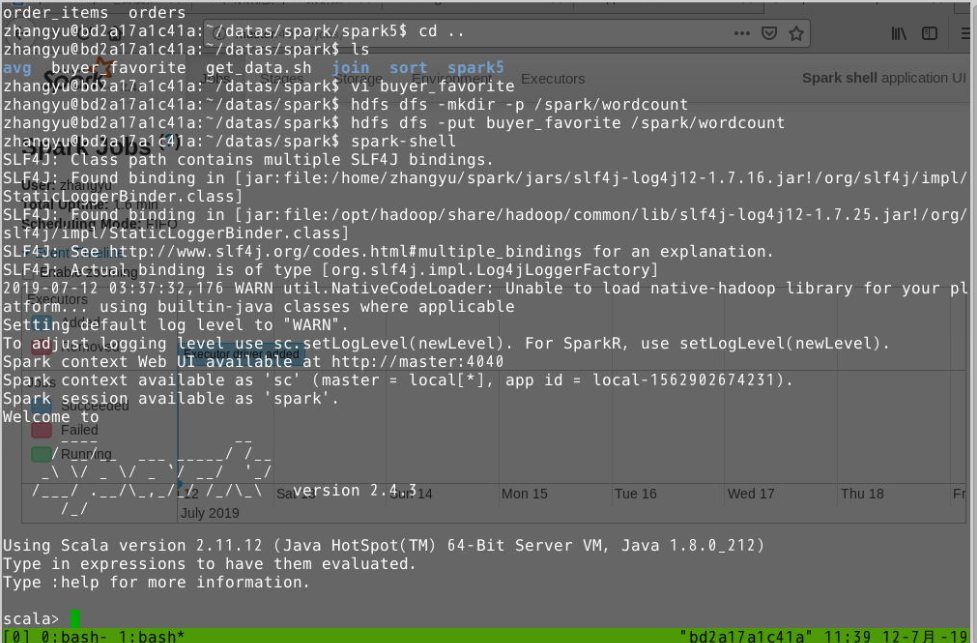
\includegraphics[width=\linewidth]{spark/spark-shell2.png}    
\end{center}
    
\begin{center}
    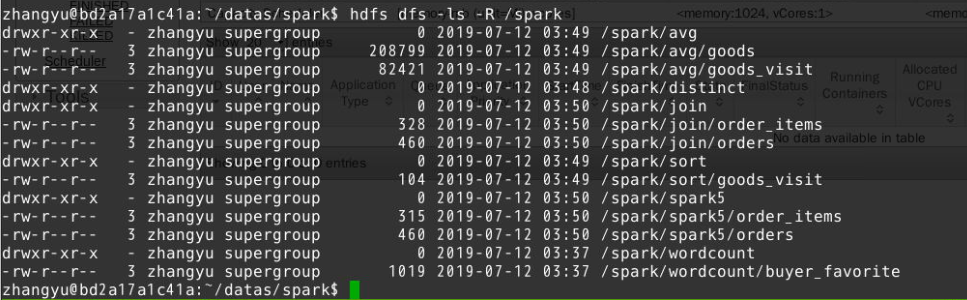
\includegraphics[width=\linewidth]{spark/test_data.png}
\end{center}

\lstinputlisting[style=mysh,title=buyer\_favorite]{docs/scripts/buyer_favorite}

\begin{center}
    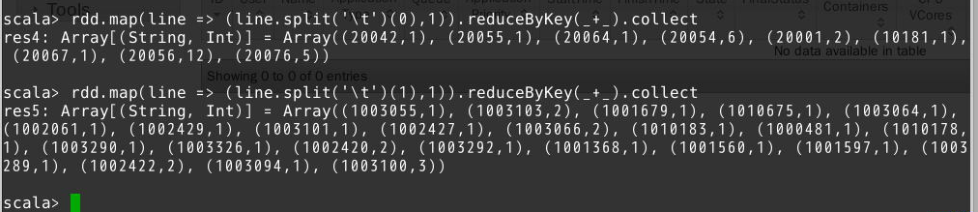
\includegraphics[width=\linewidth]{spark/wordcount.png}

    Spark实现WordCount,比Hadoop要简单的多
\end{center}
    
\begin{center}
    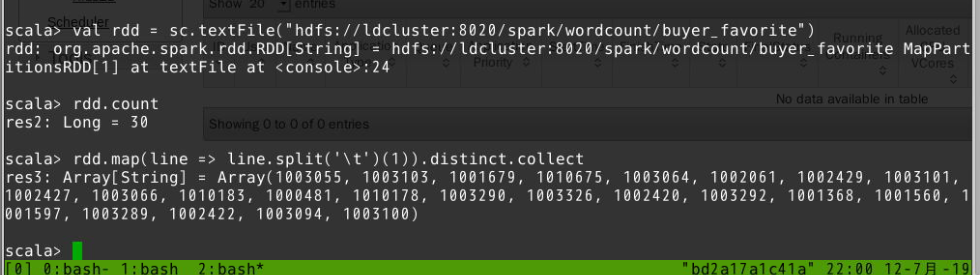
\includegraphics[width=\linewidth]{spark/rdd2.png}

    Spark实现去重,查看哪些商品被收藏
\end{center}
    
\lstinputlisting[style=mysh,title=goods\_visit]{docs/scripts/goods_visit}

\begin{center}
    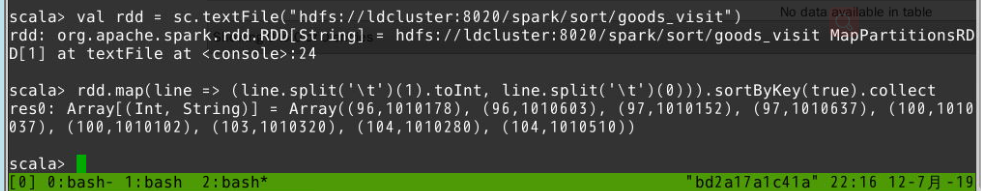
\includegraphics[width=\linewidth]{spark/rddsort.png}

    Spark对用户记录进行排序,实现按购买数升序排列。
\end{center}
    
\lstinputlisting[style=mysh,title=orders]{docs/scripts/orders}

\lstinputlisting[style=mysh,title=order\_items]{docs/scripts/order_items}

\begin{center}
    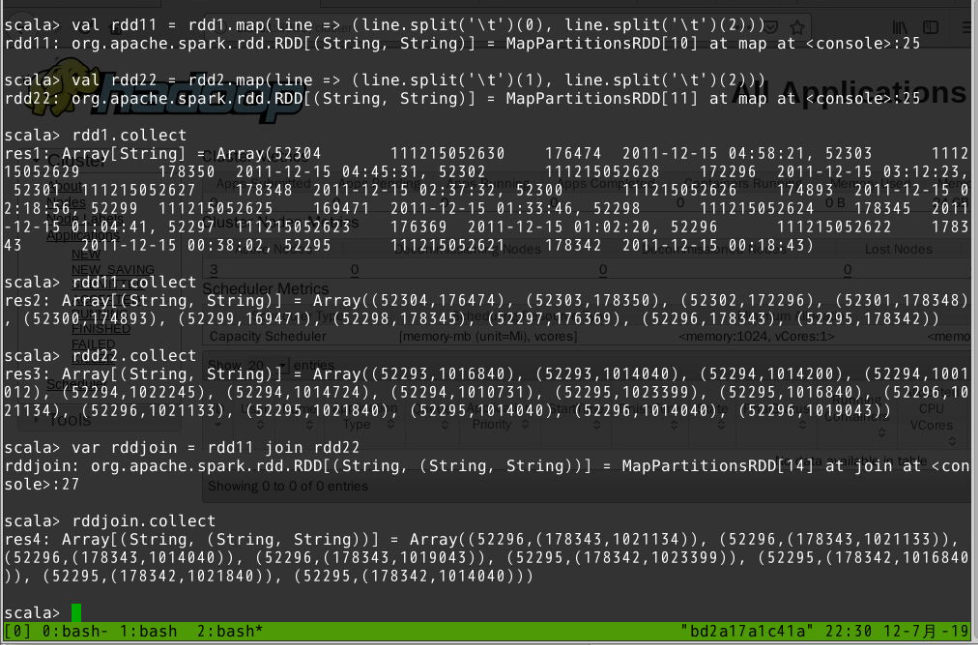
\includegraphics[width=\linewidth]{spark/rddjoin.png}

    Spark实现两张表的Join操作
\end{center}

\subsection{测试Spark SQL}

Spark SQL的前身是Shark,Shark是伯克利实验室Spark生态环境的组件之一,它能运行在Spark引擎上,从而使得SQL查询的速度得到10-100倍的提升,但是,随着Spark的发展,由于Shark对于Hive的太多依赖(如采用Hive的语法解析器、查询优化器等等),制约了Spark的One Stack Rule Them All的既定方针,制约了Spark各个组件的相互集成,所以提出了SparkSQL项目。
SparkSQL抛弃了原有Shark的代码,汲取了Shark的一些优点,如内存列存储(In-MemoryColumnarStorage)、Hive兼容性等,重新开发了SparkSQL代码;由于摆脱了对Hive的依赖性,SparkSQL无论在数据兼容、性能优化、组件扩展方面都得到了极大的方便。
SQLContext具体的执行过程如下:
\begin{figure}[htbp]
    \centering
    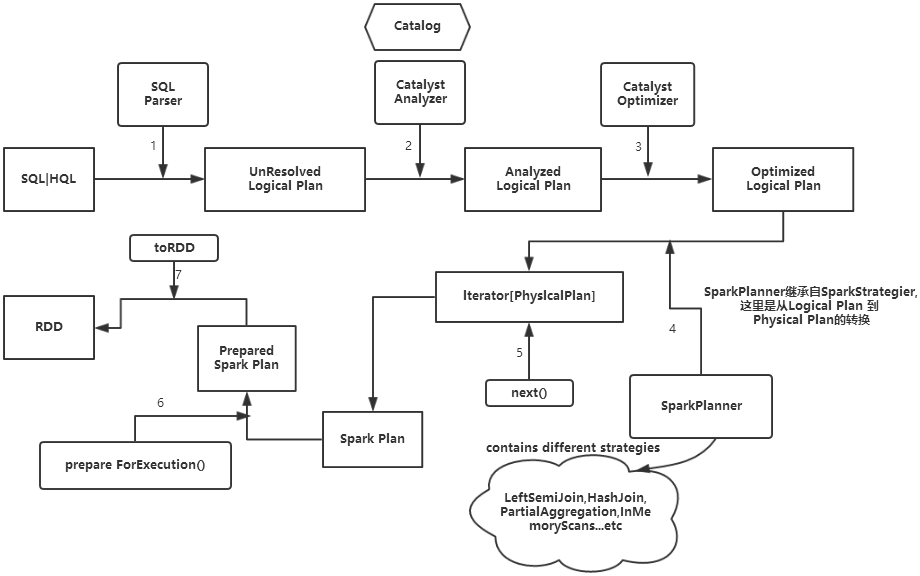
\includegraphics[width=\linewidth]{spark/spark-sql.png}
    \caption{Spark SQL执行流程}
    \label{fig:spark_sql}
\end{figure}

\begin{enumerate}[1)]
\item SQL | HQL语句经过SqlParse解析成UnresolvedLogicalPlan。
\item 使用analyzer结合数据字典(catalog)进行绑定,生成resolvedLogicalPlan,在这个过程中,Catalog提取出SchemRDD,并注册类似case class的对象,然后把表注册进内存中。
\item Analyzed Logical Plan经过Catalyst Optimizer优化器优化处理后,生成Optimized Logical Plan,该过程完成以后,以下的部分在Spark core中完成。
\item Optimized Logical Plan的结果交给SparkPlanner,然后SparkPlanner处理后交给PhysicalPlan,经过该过程后生成Spark Plan。
\item 使用SparkPlan将LogicalPlan转换成PhysicalPlan。
\item 使用prepareForExecution()将PhysicalPlan转换成可执行物理计划。
\item 使用execute()执行可执行物理计划。
\item 生成DataFrame。
\end{enumerate}
在整个运行过程中涉及到多个SparkSQL的组件,如SqlParse、analyzer、optimizer、SparkPlan等等。
\subsection{Spark Web UI}
打开浏览器可以通过http://master:4040 端口查看Spark Job的运行情况。
\begin{center}
	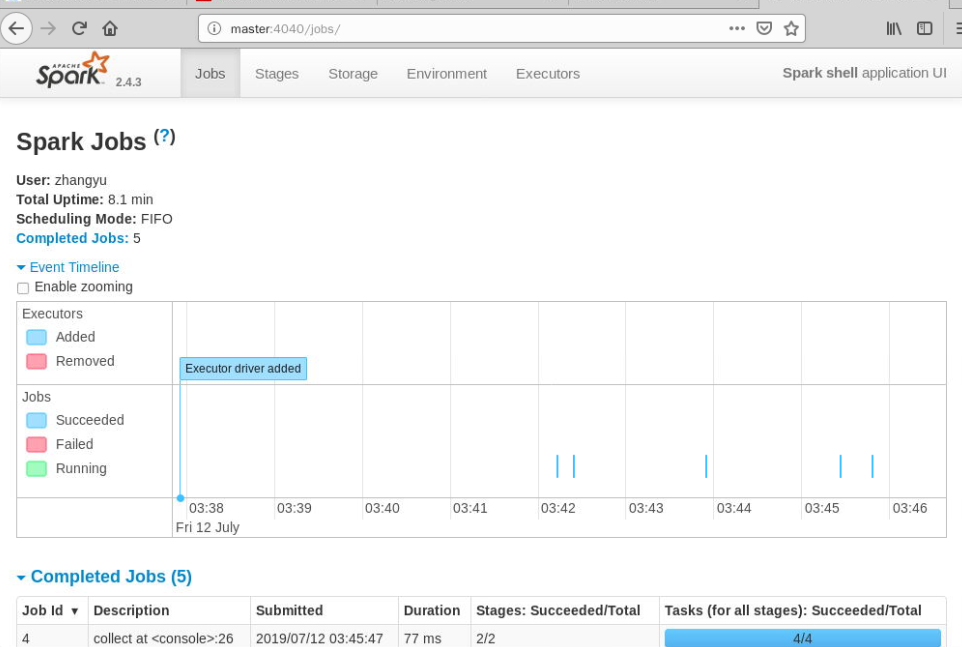
\includegraphics[width=\linewidth]{spark/sparkjobweb.png}

	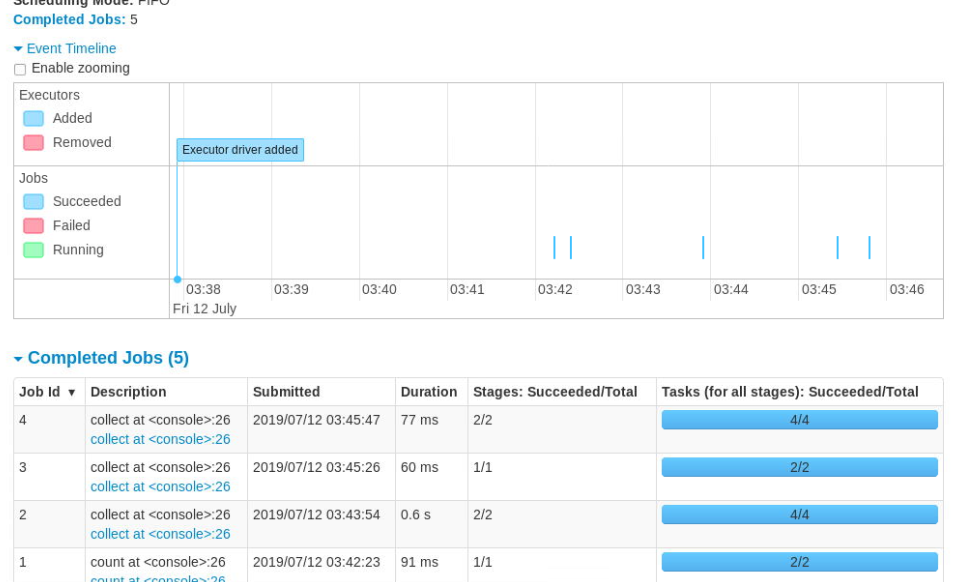
\includegraphics[width=\linewidth]{spark/sparkjobweb2.png}
\end{center}
